\chapter{设计与实现 }
\label{chp:implement}
\todo{拆封成设计实现两章}

\section{系统功能}
本文以帮助研究人员和开发人员了解Android应用程序的执行过程作为基本出发点,通过设计与实现Android动态函数调用图构建系统RunDroid,生成Android应用程序运行时对应的动态函数调用图,从方法调用关系、方法间的触发关系以及方法执行的相关对象信息等多个方面较为全面地展现Android应用的执行过程,为应用程序分析提供更为多样、准确的信息。另外,系统具备一定的可拓展性,可以方便相关人员根据自身的业务需求对系统进行扩展,完成相应的需求。

\section{基本思想}



\begin{figure*}[ht]
	\centering
	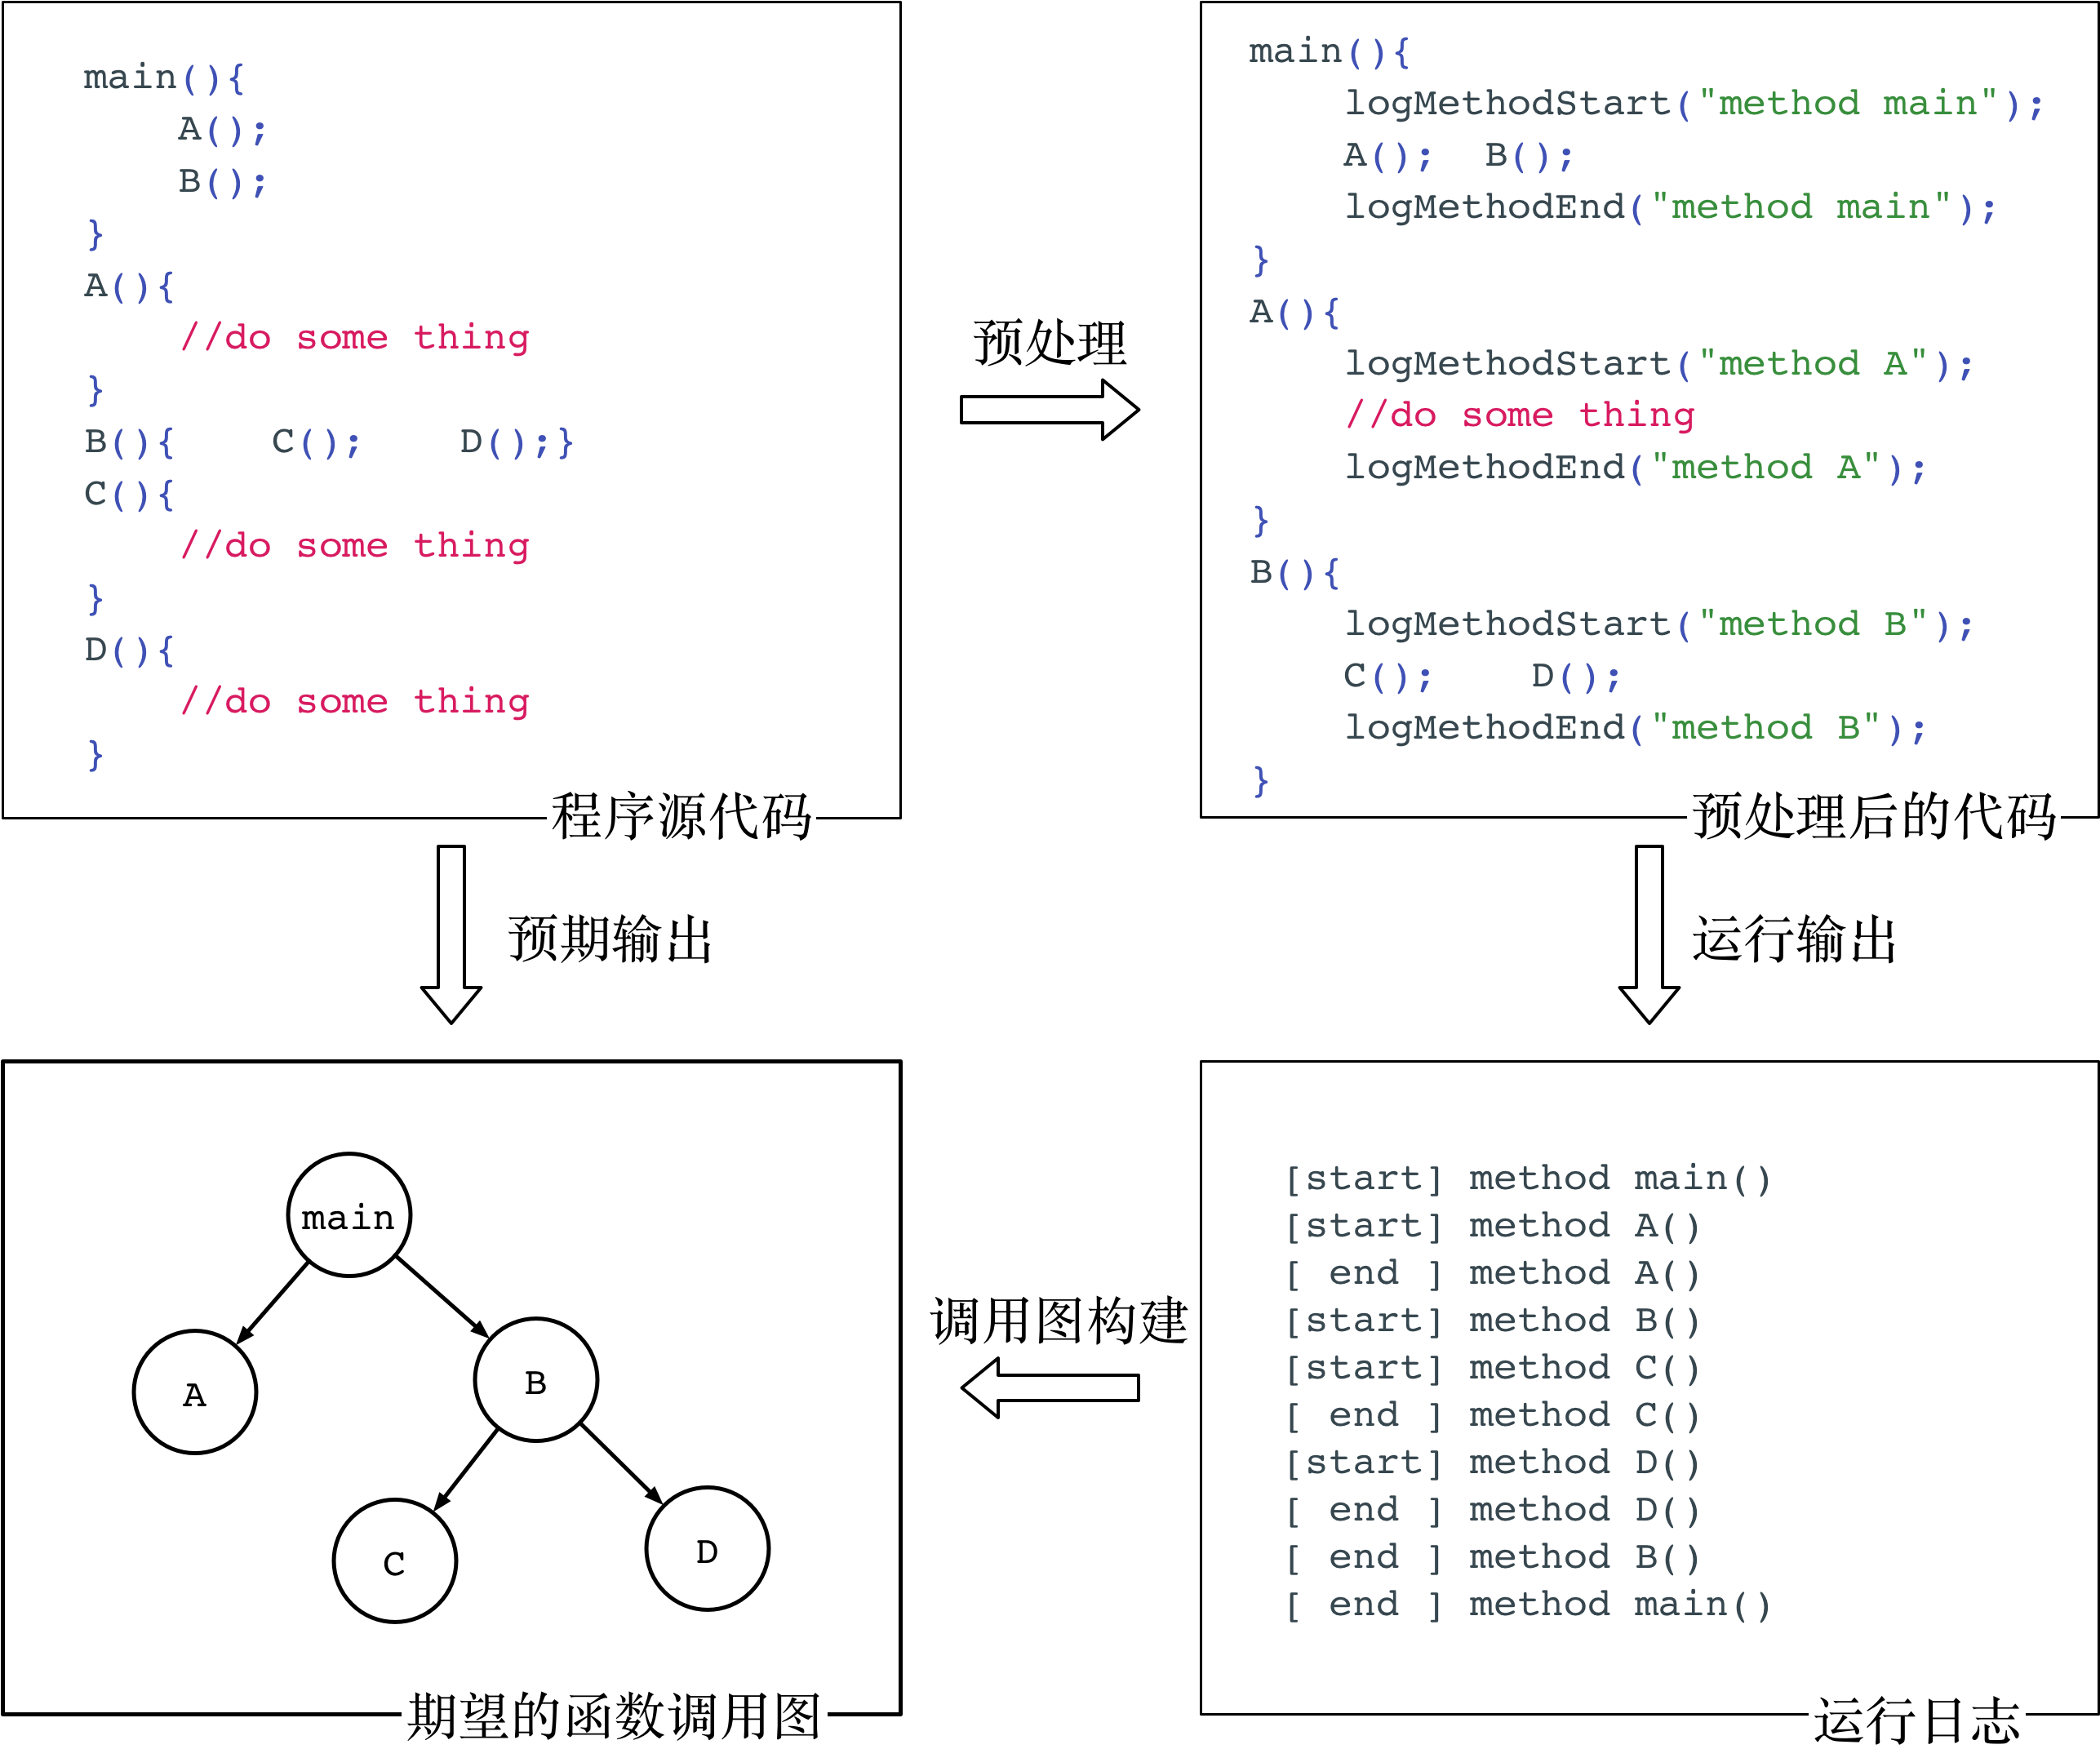
\includegraphics[width=\textwidth]{./Figures/code-sample.png}
	\caption{RunDroid的基本思路}
	\label{fig:code_sample}
\end{figure*}


%在本节,
以\autoref{fig:code_sample}为例,%简要介绍一下RunDroid还原Android应用程序的函数调用图的基本思路:
\autoref{fig:code_sample}-左上为一段示例代码:在main函数执行时,程序会依次调用A、B两个函数,而B函数则会调用了C、D两个函数。
\autoref{fig:code_sample}-左下则是期望输出——函数调用图。
在本质上,函数调用图属于树。程序执行过程可以看做树的深度优先遍历过程。
函数调用图还原的关键点,在于如何在程序执行过程中输出树的遍历序列,并根据遍历序列进行还原。
通常的,树的遍历分为中序遍历、前序遍历以及后序遍历三种。
不幸的,两颗结构完全不同的树对应的遍历序列可能是一样的,
这也就意味着上述三种遍历方法均不能直接还原出函数调用图。

若在程序执行前后均记录日志(即一个方法的执行会输出两条日志:方法开始日志、方法结束日志)时,
我们得到的遍历序列是唯一的,可以直接用于函数调用图的还原。
% 而且,函数执行过程中出现的错误异常可能使得序列输出中断,阻碍调用图的构建。

为此,我们采用的基本思路如下:
通过对源程序(\autoref{fig:code_sample}-左上)进行预处理,得到包含日志记录功能的运行代码(\autoref{fig:code_sample}-右上);
程序在函数执行前后可以输出和方法执行相关的日志信息,(\autoref{fig:code_sample}-右下);
最后,我们根据这些日志信息构建出函数调用图(\autoref{fig:code_sample}-左下)。
在函数调用图的基础上,RunDroid利用日志中包括的方法对象信息,挖掘和方法对象相关联的方法,结合具体触发规则,进而建立方法触发关系。

% 从函数调用图的构建过程可以看出,程序的执行过程就是对函数调用图自上而下的深度优先遍历过程。由此可见,若要还原出图 6-右中的函数调用图,本文采用的基本思路是以日志方式输出对右图中的函数调用图的深度优先遍历序列,并基于得到的遍历序列还原出函数调用图。
% 由于Android是由面向对象编程语言Java开发的系统,系统还需要考虑面向对象编程的特性——多态性(即同一个行为在不同的对象下的表现可以不同)。为此,RunDroid还会在函数调用图将函数执行和对应的对象进行关联,更好地体现面向对象编程的函数调用关系。基于上述的函数调用关系的信息,RunDroid根据函数调用之间的关系进一步挖掘,进一步挖掘Android系统中的特性(例如组件Activity的生命周期、多线程的交互方式)。



\section{技术路线}

在技术实现上,RunDroid主要分为预处理器、运行时拦截器、日志记录器、调用图构建器等4个部分。
对应技术路线如下:
预处理器通过源代码插桩技术实现用户方法层面的信息记录,而运行时拦截器则负责拦截系统方法的执行。
在应用运行时,日志记录器会记录用户方法和系统方法对应的执行信息,以日志的形式记录下来。
最后,调用图构建器会根据应用程序运行时输出的日志,构建拓展函数调用图。
对应的工作流程如\autoref{fig:rundroid_overview}所示。


% 本技术路线拟利用语法分析工具,对Android应用程序进行了应用源代码层面的执行日志插桩工作,利用非侵入式系统行为修改插件获取系统层面的函数执行信息。
% 结合以上日志信息,方案对日志进行初步处理,在图数据库上构建原始的Android应用程序的动态函数调用图。
% 通过阅读分析Android系统中多线程相关的源代码,制定具体的多线程分析插件,进而在函数调用图中标识出多线程相关的方法间触发关系,
%全面地展现Android应用的执行过程。


\begin{figure*}[!ht]
	\centering
	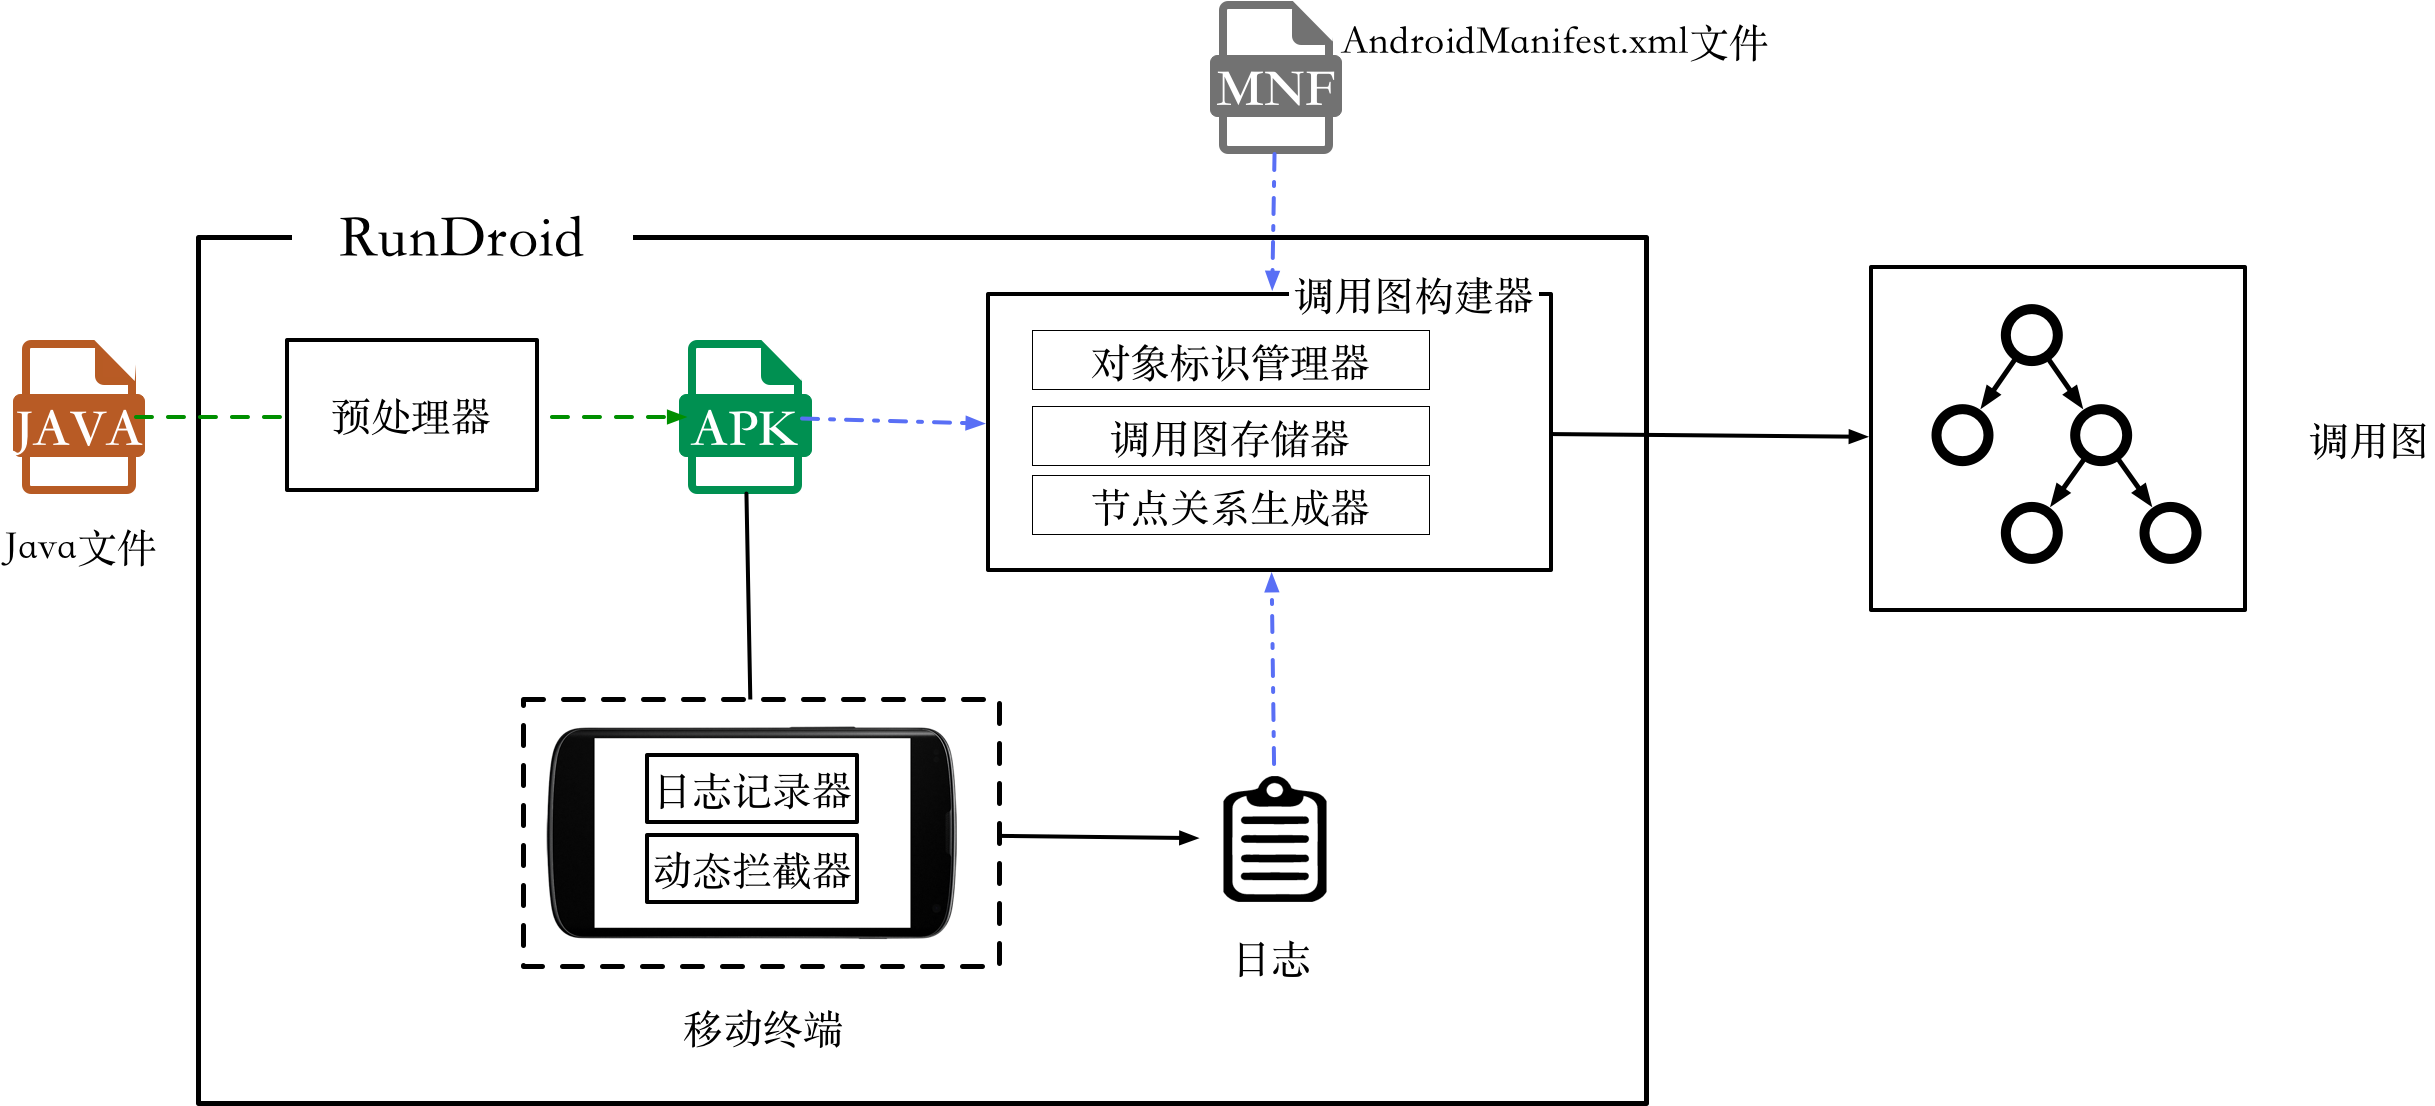
\includegraphics[height=0.7\textheight]{./Figures/rundroid-overview.png}
	\caption{ RunDroid的工作流程}
	\label{fig:rundroid_overview}
\end{figure*}


\section{相关技术介绍}


\point{srcML:}
srcML~\cite{collard2013srcml}是轻量级源代码分析工具,它可以将程序的抽象语法树以XML的形式展现给用户,支持C、C++、C\#以及Java等多个语言的语法解析。
srcML的语法解析器采用的是基于LL(*)算法实现的语法解析器 ANTLR 2.7.7,解析得到的XML内容保留了源代码中完整的语法树信息。
同时,srcML还提供了一个强大工具集,支持对生成内容的查询、分析以及修改,可以用于架构设计、语言研究、软件重构等场景,应用于软件工程、编程语言、并行和分布式处理等多个领域。
在RunDroid,srcML承担的主要职责为源代码的语法解析,辅助完成用户方法层面的日志代码的编织(weaving)。

\point{Xposed框架:}
Xposed~\cite{Xposed}是由rovo89主导开发的第三方框架。
基于Xposed开发的第三方插件,可以在不修改系统和应用程序源代码的情况下,改变他们的运行行为。
Xposed框架可以运行在不同版本的Android系统上,开发过程十分便利,而且易于撤销。
Xposed的实现原理具体如下:由于Android系统的所有的应用程序进程都是由Zygote进程孵化而来,Xposed通过替换程序\code{/system/bin/app\_process},使得系统在启动过程中加载Xposed的相关文件,将所有的目标方法指向Native方法xposedCallHandler,维护目标方法和对应的钩子方法(Hook Function)的映射关系,从而实现对Zygote进程及Dalvik虚拟机的劫持;
当程序执行到目标方法时,xposedCallHandler会完成目标方法的原有代码和对应钩子方法的调度,达到对目标方法劫持的目的。
在RunDroid中,Xposed可以帮助我们实现类似面向切面编程(Aspect-Oriented Programming, AOP)的功能,辅助完成系统方法的执行情况的日志记录。

\point{Neo4j:}
Neo4j~\cite{Neo4jthe19}是基于Java语言开发的图数据库。
与传统的基于关系模型的存储结构不同,Neo4j的存储模型是基于图论开发的,遵循属性图数据模型。
Neo4j的数据主要分为节点(Node)和关系(Relationship)两大类,分别对应图论中的点与边。
另外,Neo4j还可以在关系和节点上添加key-value形式的属性,为节点指定一个或者多个标签,为关系指定类型等等。
Neo4j以Lucence作为索引支撑,支持完整的 ACID(原子性,一致性,隔离性和持久性)事务规则,提供了基于Cypher脚本、Native Java API和REST Http API等多种方式帮助开发人员进行数据开发工作。
同时,Neo4j还提供了友好的浏览器界面,具有十分友好的交互体验。
由于基于属性图数据模型,Neo4j通常适用于和图关系有着密切关系的应用场景:例如社交网络分析,公共交通网络研究以及地图网络拓扑等场景。
在RunDroid,Neo4j主要承担着拓展函数调用图的存储、查询、展示的主要职责。

\section{模块实现}


\subsection{预处理器}

为了捕获用户方法的运行时执行信息,RunDroid的预处理器组件会对应用程序进行插桩工作。
为了避免传统字节码插桩技术在生成过多的方法数而导致的方法数65K限制问题,预处理器采用的方案是源代码层面的插桩方案。
该方案通过源程序修改,将日志记录代码直接作用在方法体内部,最大限度地减少了APK构建过程中方法数的增加,避免了方法数65K限制问题。
日志记录代码在方法执行前后会调用日志记录器输出方法执行日志。


预处理器以Android项目源代码作为输入,输出预处理后的APK文件。
预处理器会遍历项目源代码中的每一个Java文件,利用srcML转化成对应的抽象语法树。
%  利用获取的语法结构,预处理器会提取出所有的方法体,
对于抽象语法树中的每一个方法,预处理器会计算出编译后所处的类的全限类名及对应的完整的方法签名,并将这些信息以日志记录代码的形式写回到方法体中。
另外,日志记录代码记录了和方法相关的方法对象信息:和方法有参数或者实例关系的对象会在方法执行时输出到日志,方法的返回值对象则是在方法结束以后输出到日志中。
全限类名和方法签名的组合<全限类名,方法签名>和抽象语法树中的方法体一一对应,可以看做方法体的唯一标识,因此我们根据这些日志信息,定位到具体对应的方法体,还原出函数调用关系,构建出函数调用图。
另外,预处理器还对每个方法体进行了异常捕获处理,防止方法体内部的异常导日志记录过程的中断,影响函数调用图的构建。
最后,预处理器会将插桩后的源代码构建成APK文件。


\subsection{运行时拦截器}
运行时拦截器的主要职责是对Android系统定义的方法执行进行拦截,将相关信息传递给日志记录器,弥补预处理器无法捕获系统方法执行信息的缺陷。
运行时拦截器可以帮助提供系统方法的执行信息,填补调用图缺失的系统方法执行,进而可以还原出应用层和系统层之间以及系统内部的方法调用,产生完整的方法调用,进而帮助我们还原出方法间的触发关系。

在实现上,运行时拦截器是基于Xposed的插件,它维护的列表包括了所有需要拦截的系统方法(下称为目标方法),如\autoref{tbl:hookMethodList} 所示。
每当应用程序启动时,运行时拦截器通过Xposed提供的API\code{ XposedHelpers.findAndHookMethod()}将\autoref{tbl:hookMethodList}中的目标方法绑定到方法钩子(即\eat{Xposed提供的XC\_MethodHook的子类 ,}类HookCallBack)上。
在应用程序的运行过程中,HookCallBack对象的\code{beforeHookedMethod(MethodHookParam)}会在目标方法执行之前被调用,
\code{afterHookedMethod(MethodHookParam)}会在目标方法执行后调用。
最终,HookCallBack对应会将方法执行的相关信息传递给日志记录器。



\begin{table*}[!ht]
%	\centering
	%\tiny
	
	\caption{运行时拦截器拦截的系统方法列表}
	
	\label{tbl:hookMethodList}
	

	\resizebox{\textwidth}{!}{
		\begin{threeparttable}[b]
			
			\begin{tabular}{|l|c|}
				\hline
				方法签名&说明\\
				\hline
	Activity.onCreate(Bundle)   &\multirow{6}{0.4\linewidth}{和Activity生命周期相关的方法}\\
%	\cline{1-1}
	Activit. onStart()    &\\
	Activity.onResume()     &\\
	Activity.onPause()    &\\	
	Activity.onStop()     &\\
	Activity.onDestroy()    &\\
				\hline
				
				Thread start   & 和Java 线程启动相关的方法\\
				\hline
				Message.obtain() & \multirow{15}{0.4\linewidth}{和 Hanlder机制相关的方法}\\
				Handler.enqueueMessage(MessageQueue,Message,long)&\\
				Handler.dispatchMessage(Message)&\\
				Handler.post(Runnable)&\\
				Handler.postAtTime(Runnable,long)&\\
				Handler.postAtTime(Runnable,Object,long)&\\
				Handler.postDelayed(Runnable,long)&\\
				Handler.postAtFrontOfQueue(Runnable)&\\
				Handler.sendMessage(Message)&\\
				Handler.sendEmptyMessage(int)&\\
				Handler.sendEmptyMessageDelayed(int,long)&\\
				Handler.sendEmptyMessageAtTime(int,long)&\\
				Handler.sendMessageAtFrontOfQueue(Message)&\\
				Handler.sendMessageDelayed(Message,long)&\\
				Handler.sendMessageAtTime(Message,long)&\\
				
				\hline
 
				
		%		AsyncTask execute [Object& \multirow{3}{0.4\linewidth}{和 AsyncTask相关的方法}\\
		%		AsyncTask publishProgress [Object&\\
		%		AsyncTask executeOnExecutor Executor [Object &\\
		%		\hline
 
				
			\end{tabular}
		
%		\begin{tablenote}
	%		\end{tablenote}
			
		\end{threeparttable}
	}
\end{table*}




%   进而通过日志记录器输出相应的日志。


% 拦截器组件基于Xposed框架[5],它拦截在应用程序层和Android框架之间传递的消息。
 % 拦截器记录在两个层之间进行的每个方法调用,并将它们与应用程序层中对应的方法调用相关联,以产生完整的方法调用跟踪。
 % RunDroid维护感兴趣的方法列表,如生命周期方法和隐式回调,以便日志文件包含每次执行期间调用的方法调用




\subsection{日志记录器}

日志记录器的职责是将方法执行的消息以日志的形式就持久化下来。
针对不同的方法类型(静态方法与非静态方法、用户方法与系统方法等),日志记录器提供了不同的API,帮助我们记录相应方法执行的日志信息。
在日志内容上,日志记录器还会记录每个方法执行的所处线程、方法签名标识、所处阶段(开始执行该方法/方法执行完毕)以及相关的方法对象信息(包括对象的类型、基本属性以及内存地址等)。
% 在底层实现上,考虑日志读入文件对程序执行效率的影响,我们评估了多种日志写入方式,最终我们发现基于mmap的日志记录方式效率最高,对程序运行的影响最小。


 \subsection{调用图构建器}

拓展函数调用图构建器(以下简称调用图构建器)的主要功能是拓展函数调用图的构建、存储和展现。
在实现上,调用图构建器主要有以下几个部分组成:对象标识管理器、调用图存储器以及触发关系生成器。

调用图构建器以应用程序在运行时的日志信息作为输入,利用日志中的方法执行信息在调用图储存器中初步建立函数调用图。
同时,对象标识管理器会根据对象使用的上下文(如该和哪个方法产生关联,具体的关系是什么等)赋予相应的标识ID,并将其添加到函数调用图中。
最后,根据调用图储存器中方法和对象之间的关系结合具体的触发关系,触发关系生成器会还原出方法间的函数触发关系。
% RunDroid通过动态执行跟踪匹配这些调用来应对这个挑战,这导致开发三个子组件:引用存储库组件、映射引擎组件、合成器组件。
% Reference Repository组件构建于Neo4j[4]之上,它处理日志文件,并存储捕获的方法及其执行调用。
% Mapping Engine组件构建于soot[13]之上,从日志历史中识别异步调用对,搜索它们相应的实例化类,并将这些捕获的多线程方法调用存储为“触发器”关系。
% 然后,Synthesizer组件将这些触发器关系与捕获的执行调用集成到一个完整的执行调用跟踪中,并存储在Reference Repository中。
在技术选型上,调用图存储器采用Neo4j作为调用图的底层存储引擎,触发关系生成器中的规则定义由Cypher脚本和Soot共同实现。


\section{基于源代码的日志代码插桩过程}
\todo{xxxx\autoref{alg:instrument}}


\begin{algorithm}[!ht]
	\caption{函数调用图的构建过程} 
	\label{alg:instrument}
	\KwIn{ $logs$,应用程序的运行时日志}
	\KwOut{ $cg$,函数调用图}
	\SetKwProg{Fn}{Function}{:}{}
	
	\Fn{buildCallGraph($log$)}{
		
		$cg$ $\gets$ new CallGraph();
		
		\KwResult{new Java File }
	}
	
\end{algorithm}

\section{扩展函数调用图的构建过程}

调用图构建器构建拓展函数调用图的过程分为两个阶段:RunDroid根据程序运行时的日志提取函数间的调用关系,创建函数调用图;
在函数调用图的基础上,RunDroid利用方法执行与方法对象的关联关系,结合具体的触发关系规则,创建方法间的触发关系,形成最终的拓展函数调用图。


\begin{algorithm}[!ht]
	\caption{函数调用图的构建过程} 
	\label{alg:buildCG}
	\KwIn{ $logs$,应用程序的运行时日志}
	\KwOut{ $cg$,函数调用图}
	\SetKwProg{Fn}{Function}{:}{}
	
	\Fn{buildCallGraph($log$)}{
		
		$cg$ $\gets$ new CallGraph();
		
		\For{thread $\in$ $logs.threads$}{
			
			$stack$ $\gets$ new Stack();
			
			\For  {$log$ $\in$ $logs.get(thread)$}{
				
				$top$ = $stack$.peek() ;  
				
				\eIf{isMethodStartLog($log$)} {
					
					$m \gets $ generateMethodInfo($log$);
					
					$cg$.addMethodNode($m$);
					%\Comment 在调用图中提交方法节点 
					
					$cg$.addMethodObjects($ o_p $,$o_i $) 	;							
					
					$cg$.addMethodObjectRels($ \left\langle  o_p \joinrel\xrightarrow{parameter}   m \right\rangle   $,$ \left\langle  o_i \joinrel\xrightarrow{instance}   m \right\rangle  $) ;
					
					%	\Comment 在调用图中提交方法对象节点 (此处只涉及参数关系和实例关系)
					
					\If {  $top \neq null $ }{
						
						$cg$.addInvokeRel($ \left\langle  top \to  m \right\rangle  $) ;
						
						$stack$.push($m$);
					}
					
				}{ 
					
					$cg$.addMethodObject($  o_r  $) ;
					
					$cg$.addMethodObjectRel($ \left\langle   o_r \joinrel\xrightarrow{return}   m \right\rangle  $) ;
					
					%		  \Comment 在调用图中提交方法对象节点 (此处只涉及返回值关系)
					
					$stack$.pop() ;
					
				}
				
				
				
			}
		}
	}
	
\end{algorithm}

\subsection{构建函数调用图}

%虽然所有线程的方法日志输入到同一个文件中,但是,从单个线程的视角看这些日志,日志在时间维度上的先后顺序就是对调用图的深度遍历。
%已检测的应用程序将日志输出到单个文件中。
%虽然所有线程的日志都输出到一个日志文件中,但在每个线程的视图中,日志条目的输出顺序遵循调用图的顺序遍历:调用方法在被调用方法之前输出。
%此外,每个方法执行对应于两个日志条目:方法入口和出口的日志条目。

由于各个线程在执行过程中,不存在一个调用关系跨越两个线程,因此,在整个构建过程中,RunDroid以产生日志的线程为基本构建单元,向调用图添加方法调用关系。
函数调用图的构建过程如\autoref{alg:buildCG}所示。
对于每个线程,RunDroid顺序遍历对应的日志,使用栈$stack$的入栈、出栈操作来模拟对应线程的函数执行的过程,还原调用关系(第3$\sim$ 20行):
当读取到方法执行的开始日志时,系统会在调用图创建一个节点表示该方法的执行(第7$\sim$8行),
同时也在调用图中添加方法参数、方法实例对应的对象节点$o_p$、$o_i$以及方法对象和方法的关系$ \left\langle  o_p \joinrel\xrightarrow{parameter}   m \right\rangle   $、$ \left\langle   o_i \joinrel\xrightarrow{instance}   m \right\rangle  $(第9$\sim$10行)。
如果此时当前线程栈$stack$的栈顶方法元素$top$存在,系统会创建从方法$top$到当前方法$m$的调用关系,$\left\langle top \to m \right \rangle  $,并将当前方法$m$压入栈$stack$中(第11$\sim$ 14行)。
当读取到方法执行的结束日志时,该日志对应的方法必然是栈顶方法$top$,若栈顶方法$top$存在返回对象$o_r$,则只需要将$o_r$和$top$的关系添加到调用图中即可,最后弹出栈顶的$top$即可(第 16$\sim$ 18行)。
在上述过程中,如果待添加的方法对象在调用图中已经存在时,该对象则无须重新添加,只需添加方法与对象间的关系即可。


% 当日志条目表示方法条目时,将根据日志条目和来自的4元组信息创建节点 日志存储在节点中(第6行)。
%然后,从堆栈顶部的方法到日志条目中的方法(第7-9行)构建调用关系。
%处理完调用关系后,该方法将被推入堆栈。当日志条目表示方法退出时,堆栈将弹出顶部的方法节点(第11-12行)。
%重复该过程,直到没有为一个线程留下日志条目,然后将为日志文件中的另一个线程启动相同的进程。

%构建扩展调用图。 
%DROIDSTITCHER通过添加表示已识别触发关系的边来扩展调用图。
%请注意,触发器关系中的目标方法通常是回调方法的调用图的入口点。
%因此,通过将触发关系添加为边,将所有调用图拼接成一个调用图作为输出。



\subsection{构建Activity的生命周期}

Android Acticvity生命周期的构建利用的是\code{Activity}生命周期相关方法的签名的不变性。
具体过程如下:
遍历调用图中所有的方法,如果一个方法的方法签名属于第\ref{chp:background}章中\autoref{fig:Activity-lifecycle}定义的方法,并且这个方法在调用图中不在调用者\footnote{不允许调用者存在是为了防止误判下面这种情况:开发人员在重写生命周期方法时调用了父类的生命周期方法。},执行线程为主线程,则这些线程为Activity生命周期的相关方法。
将上述方法按照时间顺序连接起来,即可得到\code{Activity}的生命周期。

 \subsection{构建多线程触发关系}
在构建多线程触发关系时,我们只要分为两个方面:基于Java 的多线程交互与基于\code{Handler} 的多线程消息调度。具体的过程如\autoref{alg:buildTrigger}所示。

\point{基于Java 的多线程交互}

基于Java的多线程交互往往是以\code{Runnable}作为传递对象,通常通过调用方法\code{Thread.start()} (用$m_{start}$表示)和\code{Activity.runOnUiThread(Runnable)}(用$m_{runOnUiThread}$表示)等API,进而触发方法\code{Runnable.run()}(用$m_{run}$表示)的执行。
因此,对于方法\code{Thread.start()},如果存在一个\code{Runnable}类型的对象\code{r},它既是方法$m_{start}$的实例,又是方法$m_{run}$的实例,则两个方法间存在触发关系,即$m_{start} \hookrightarrow m_{run}$(第8 $\sim$10行)。
同样的,对于方法\code{Activity.runOnUiThread(Runnable)},也存在类似的关系:
如果存在一个\code{Runnable}类型的对象\code{r},它既是方法$m_{runOnUiThread}$的参数,又是方法$m_{run}$的实例,则两个方法间存在触发关系,即$m_{runOnUiThread} \hookrightarrow m_{run}$(第11 $\sim$13行)。

\eat{\begin{equation}
	\label{equ:rule_1}
	\left. \begin{gathered}
	o_r    \        is           \      Runnable  \      Class \\
	rel(m_{start}, o_r) = instance \\
	rel(m_{run}, o_r) = instance \\
	\end{gathered} \right\}
	\Rightarrow  m_{start} \hookrightarrow m_{run}. 
	\end{equation}
}
\eat{
\begin{equation}
\label{equ:rule_2}
\left. \begin{gathered}
o_r    \        is           \      Runnable  \      Class \\
rel(m_{runOnUiThread}, o_r) = parameter \\
rel(m_{run}, o_r) = instance \\
\end{gathered} \right\}
\Rightarrow  m_{runOnUiThread} \hookrightarrow m_{run}. 
\end{equation}
}





\begin{algorithm}[!ht]
	\caption{扩展函数调用图的构建过程}
	\label{alg:buildTrigger}
	\KwIn {	$cg$, 函数调用图} 
	\KwOut {	$ecg$,拓展函数调用图}

	
	\SetKwProg{Fn}{Function}{:}{}
	\Fn{buildExtendedCallGraph($cg$)}{
		
		$ecg \gets cg$;
		
		addThreadTrigger($ecg$);
		
		addHandlerTrigger($ecg$);
		
		\KwRet $ecg$;
	}

% $o_p \stackrel{parameter}{\longrightarrow} m$
	\Fn{addThreadTrigger($ecg$)} {
		\For{\emph{$o_r \in \{ o \mid o$  is the $Runnable$ object node $\in$ $ecg \}$} }{
			\If{ $ \left\langle m_{start}\joinrel\xrightarrow{instance} o_r \right\rangle \in ecg$  \\\qquad 
					and   $\left\langle m_{run} \joinrel\xrightarrow{instance}   o_r\right\rangle  \in ecg$ }{
				$ecg$.addThreadTriggerRel($m_{start} \hookrightarrow m_{run} $)	
			}
			\If{ $ \left\langle m_{runOnUiThread} \joinrel\xrightarrow{parameter}   o_r \right\rangle \in ecg$  \\\qquad   
				and   $\left\langle m_{run} \joinrel\xrightarrow{instance}   o_r\right\rangle  \in ecg$  }{
				$ecg$.addThreadTriggerRel($m_{runOnUiThread} \hookrightarrow m_{run} $)	
			}	
		}
	}	
	\Fn{addHandlerTrigger($ecg$)} {
		
		\For{\emph{ $o_m \in  \{ o\mid$ o is the $Message$ object node $\in$ $ecg \}$} }{
				\If{ $ \left\langle m_{enqueue}\joinrel\xrightarrow{parameter} o_m\right\rangle \in ecg$  \\\qquad   
					and   $\left\langle m_{dispatch}\joinrel\xrightarrow{parameter} o_m\right\rangle  \in ecg$ }{
						$m_{send}$ =  calculateSendMethod($ecg$,$m_{enqueue}$);
						
						$m_{handle}$ =  calculateHandleMethod($ecg$,$m_{dispatch}$);
						
						$ecg$.addHandleTriggerRel($m_{send} \hookrightarrow m_{handle} $)	
				}	
		}
	}
	
\end{algorithm}





\point{基于\code{Handler} 的多线程消息调度}

根据第\ref{chp:background}、\ref{chp:definition}章的介绍,我们已经知晓用户通过调用Handler提供的API,
将相关业务逻辑借助Message对象传递给目标线程的Handler对象,在目标线程执行相应的业务逻辑处理。
%在这个部分,我们需要找出用户调用的Handler API和对应目标线程的业务逻辑方法间的触发关系:

首先,我们利用handler的方法\code{enqueueMessage(Message)}(用$m_{enqueue}$表示)和\code{dispatchMessage(Message)}(用$m_{dispatch}$表示)公用同一个Message对象的特点,
找到所有的Handler底层函数触发关系 ,$m_{enqueue}  \hookrightarrow  m_{dispatch}$ (第16$\sim$17 行);
对于每一个触发关系 $m_{enqueue}  \hookrightarrow  m_{dispatch}$,
从$m_{enqueue}$ 顺着调用关系往上找到最上层的Handler API方法(即用户调用的Handler API方法,$m_{send}$)(第18行),
从$m_{dispatch}$ 顺着调用关系往下找到用户定义的方法\code{Handler.handleMessage(Message)}$m_{handle}$(第19行),
最后在调用图中提交方法$m_{send}$和$m_{handle}$之间的触发关系 $m_{send} \hookrightarrow m_{handle}$(第20行)。
%如果$m_{send}$和$m_{handle}$中有一个方法未找到,表示


\eat{
MATCH (SEND:METHOD)-[:PARAM]->(MSG:OBJECT),

(SEND:METHOD)-[:INSTANCE]->(HANDLER:OBJECT),

(HANDLE:METHOD)-[:PARAM]->(MSG:OBJECT),

(HANDLE:METHOD)-[:INSTANCE]->(HANDLER:OBJECT)

WHERE SEND.methodSign ='boolean android.os.Handler.enqueueMessage(android.os.MessageQueue,android.os.Message,long)'

AND HANDLE.methodSign ='void android.os.Handler.dispatchMessage(android.os.Message)'

RETURN SEND,HANDLE
	
	
	
	
MATCH p=(method:METHOD)-[:INVOKE*0..]->(enqueue:METHOD),

(enqueue)-[:TRIGGER\_PREPARE\_HANDLER]->(dispatch:METHOD)

AND  NOT (enqueue)-[:INVOKE]->()

RETURN p,method,enqueue,dispatch;

	
	
MATCH p=(method:METHOD)-[:INVOKE*0..]->(enqueue:METHOD),

(enqueue)-[:TRIGGER\_PREPARE\_HANDLER]->(dispatch:METHOD)-[r:INVOKE]->(run:METHOD)

WHERE method.methodSign IN [

'boolean android.os.Handler.post(java.lang.Runnable)',

'boolean android.os.Handler.postAtTime(java.lang.Runnable,long)',

'boolean android.os.Handler.postAtTime(java.lang.Runnable,java.lang.Object,long)',

'boolean android.os.Handler.postDelayed(java.lang.Runnable,long)']

RETURN p,method,enqueue,dispatch, run

	
	
	
MATCH p=(method:METHOD)-[:INVOKE*0..]->(enqueue:METHOD),

(enqueue)-[:TRIGGER\_PREPARE\_HANDLER]->(dispatch:METHOD)

AND  NOT (enqueue)-[:INVOKE]->()

RETURN p,method,enqueue,dispatch

	

}

\eat{识别触发关系。
触发关系表示由于Android框架的生命周期事件,系统事件和多线程通信而导致的方法的隐式调用。
以Handler为例。 sendMessage方法隐式意味着稍后将执行相应的方法handlerMessage。
为了捕获这种关系,我们确定了一种模式:sendMessage方法通过传递消息对象来触发方法handlerMessage。
因此,如果我们可以找到用作方法sendMessage和方法handlerMessage的参数的消息对象,那么我们可以在这两个方法之间创建触发器关系。
在分析了Android框架的源代码之后,我们确定了线程,窗口小部件的侦听器注册和异步任务的类似模式。
因此,DROIDSTITCHER维护一个方法列表,这些方法是触发器关系的潜在目标,并比较这些方法中消息对象的内存地址以推断关系。
}
 \section{本章小结}

本章详细介绍了RunDroid的设计与实现。
首先,本章简要介绍了RunDroid实现的基本功能,并通过一个简单的例子介绍了RunDroid运行的基本思路。
由此,我们提出了RunDroid具体的技术路线:RunDroid利用源代码插桩和运行时拦截器相结合的方式,将运行时的方法执行信息以日志的形式保存下来,通过线程内部各个方法日志的嵌套关系还原出函数调用图,并利用调用图中方法和方法对象之间的关系结合具体的触发关系补全方法间的触发关系,形成最终的拓展函数调用图。
此外,我们还介绍了RunDroid在实现上使用到的技术以及各模块的具体实现。
